%%-----------------------------------------------------------------------
%% Make your own quadrille, graph, hex, etc paper!
%% Uses the pgf/TikZ package for LaTeX, which should be part of
%% any modern TeX installation.
%%
%% All the values here are hardcoded for letter size paper. 
%%
%% This is the original standalone .tex file. The project is in the
%% process of being converted to a LaTeX package.
%%
%% Github: https://github.com/mcnees/LaTeX-Graph-Paper
%% 
%% Email: mcnees@gmail.com
%% Twitter: @mcnees
%%
%% Last Update: 2/18/21 - Added triangle and isometric fills
%%-----------------------------------------------------------------------
\documentclass[11pt]{article}

%%-----------------------------------------------------------------------
%% This package gives small margins so you use less
%% paper.
%%-----------------------------------------------------------------------
\usepackage[cm]{fullpage}

%%-----------------------------------------------------------------------
%% Packages needed for the drawing routines and for mixing custom
%% colors.
%%-----------------------------------------------------------------------
\usepackage{tikz}
\usetikzlibrary{patterns}
\usepackage{xcolor}

%%-----------------------------------------------------------------------
%% A package for setting the background color of the page
%%-----------------------------------------------------------------------
\usepackage{pagecolor}

%%-----------------------------------------------------------------------
%% Which pattern style do we want?
%%-----------------------------------------------------------------------
%% Names of patterns. These are basically enum values because I don't
%% know how to really program in TeX.
\def\stdpat       		{std}        % Standard, ten squares per inch (s.p.i.)
\def\stdeightpat 		{stdeight}   % Standard, eight s.p.i.
\def\majminpat    		{majmin}     % Eight s.p.i. w/ major grid ever 1/2 inch
\def\dotpat       		{dot}        % Dot grid
\def\hexpat      		{hex}        % Hex grid
\def\tripat          	{tri}        % Triangle grid
\def\isopat          	{iso}        % Isometric grid
\def\lightconepat 		{lightcone}  % Light cone grid
\def\ruledpat     		{ruled} 	   % Ruled paper
\def\doubleruledpat     {doubleruled} 	   % Ruled paper

%% Which pattern style to use. CHOOSE HERE by using one of the magic
%% tokens above: std, stdeight, majmin, dot, hex, lightcone
\def\usepat{majmin}

%%-----------------------------------------------------------------------
%% Some nice colors.
%%-----------------------------------------------------------------------
\definecolor{plum}{rgb}{0.36078, 0.20784, 0.4}
\definecolor{chameleon}{rgb}{0.30588, 0.60392, 0.023529}
\definecolor{cornflower}{rgb}{0.12549, 0.29020, 0.52941}
\definecolor{scarlet}{rgb}{0.8, 0, 0}
\definecolor{brick}{rgb}{0.64314, 0, 0}
\definecolor{sunrise}{rgb}{0.80784, 0.36078, 0}
\definecolor{rosiebg}{RGB}{250,247,232}
\definecolor{rosiegrid}{RGB}{186,137,113}


%%-----------------------------------------------------------------------
%% Pre-defined Color schemes
%%-----------------------------------------------------------------------
%% Here are some pre-defined color schemes for the paper background
%% and the major and minor gridlines. Simply uncomment the "\colorlet"
%% lines below. 
%%
%% A number of rgb colors are defined above. You can make either one 
%% darker by changing the number after the "!". For instance, 
%% cornflower!75 is darker than cornflower!25.

% Blue lines on white background
\colorlet{minorcolor}{cornflower!30}
\colorlet{majorcolor}{cornflower!50}
\colorlet{bgcolor}{white}

% % Precocious Engineer
% \colorlet{minorcolor}{rosiegrid!50}
% \colorlet{majorcolor}{rosiegrid}
% \colorlet{bgcolor}{rosiebg}

%% Red paper
% \colorlet{minorcolor}{brick!35}
% \colorlet{majorcolor}{brick!60}
% \colorlet{bgcolor}{scarlet!8}

% % Engineer Pad
% \colorlet{minorcolor}{chameleon!50}
% \colorlet{majorcolor}{chameleon!80}
% \colorlet{bgcolor}{chameleon!10}

%% Plum pad
% \colorlet{minorcolor}{cornflower!40}
% \colorlet{majorcolor}{cornflower!70}
% \colorlet{bgcolor}{plum!10}

%%-----------------------------------------------------------------------
%% The color to use for the null directions when drawing lightcones.
%%-----------------------------------------------------------------------
\colorlet{lightlines}{scarlet!30}


%%-----------------------------------------------------------------------
%% This section sets up a routine for filling a shape with
%% hexagons. Uses code from:
%% http://tex.stackexchange.com/questions/6019/drawing-hexagons/6128#6128
%%-----------------------------------------------------------------------

%% Uncomment one of the two "\def" lines below for Big or Small hexagons.
%% Big hexagons
\def\hexagonsize{0.1666in}
%% Small hexagons
%\def\hexagonsize{0.0833in}

\pgfdeclarepatternformonly
  {hexagons}% name
  {\pgfpointorigin}% lower left
  {\pgfpoint{3*\hexagonsize}{0.866025*2*\hexagonsize}}
  {\pgfpoint{3*\hexagonsize}{0.866025*2*\hexagonsize}}
  {
    \pgfsetlinewidth{0.6pt}
    \pgftransformshift{\pgfpoint{0mm}{0.866025*\hexagonsize}}
    \pgfpathmoveto{\pgfpoint{0mm}{0mm}}
    \pgfpathlineto{\pgfpoint{0.5*\hexagonsize}{0mm}}
    \pgfpathlineto{\pgfpoint{\hexagonsize}{-0.866025*\hexagonsize}}
    \pgfpathlineto{\pgfpoint{2*\hexagonsize}{-0.866025*\hexagonsize}}
    \pgfpathlineto{\pgfpoint{2.5*\hexagonsize}{0mm}}
    \pgfpathlineto{\pgfpoint{3*\hexagonsize}{0mm}}
    \pgfpathmoveto{\pgfpoint{0.5*\hexagonsize}{0mm}}
    \pgfpathlineto{\pgfpoint{\hexagonsize}{0.866025*\hexagonsize}}
    \pgfpathlineto{\pgfpoint{2*\hexagonsize}{0.866025*\hexagonsize}}
    \pgfpathlineto{\pgfpoint{2.5*\hexagonsize}{0mm}}
    \pgfusepath{stroke}
  }

%%-----------------------------------------------------------------------
%% This section sets up a routine for filling a shape with
%% triangles.
%%-----------------------------------------------------------------------

%% Uncomment one of the two "\def" lines below for Big or Small triangles.
% Bigger triangles
\def\trianglesize{2*0.125in}
% Smaller triangles
%\def\trianglesize{0.125in}

\pgfdeclarepatternformonly
  % Name of the pattern
  {triangles}
  % Set the lower left corner of the pattern
  {\pgfpointorigin}
  % Set the upper right corner of the pattern
  {\pgfpoint{\trianglesize}{2*0.8660254*\trianglesize}}
  % Declare the size of the pattern blocks
  {\pgfpoint{\trianglesize}{2*0.8660254*\trianglesize}}
  % Draw the pattern
  {
    \pgfsetlinewidth{0.6pt}
	\pgfpathmoveto{\pgfpoint{0mm}{0mm}}
	\pgfpathlineto{\pgfpoint{\trianglesize}{2*0.8660254*\trianglesize}}
	\pgfpathlineto{\pgfpoint{0mm}{2*0.8660254*\trianglesize}}
    \pgfpathmoveto{\pgfpoint{0mm}{0.8660254*\trianglesize}}
	\pgfpathlineto{\pgfpoint{\trianglesize}{0.8660254*\trianglesize}}
    \pgfpathmoveto{\pgfpoint{0mm}{2*0.8660254*\trianglesize}}
	\pgfpathlineto{\pgfpoint{\trianglesize}{0mm}}
	\pgfpathlineto{\pgfpoint{0mm}{0mm}}
    \pgfusepath{stroke}
  }
  
\pgfdeclarepatternformonly
  % Name of the pattern
  {isometric}
  % Set the lower left corner of the pattern
  {\pgfpointorigin}
  % Set the upper right corner of the pattern
  {\pgfpoint{2*0.8660254*\trianglesize}{\trianglesize}}
  % Declare the size of the pattern blocks
  {\pgfpoint{2*0.8660254*\trianglesize}{\trianglesize}}
  % Draw the pattern
  {
    \pgfsetlinewidth{0.6pt}
	\pgfpathmoveto{\pgfpoint{0mm}{0mm}}
	\pgfpathlineto{\pgfpoint{2*0.8660254*\trianglesize}{\trianglesize}}
	\pgfpathlineto{\pgfpoint{2*0.8660254*\trianglesize}{0mm}}
	\pgfpathlineto{\pgfpoint{0mm}{\trianglesize}}
	\pgfpathlineto{\pgfpoint{0mm}{0mm}}
    \pgfpathmoveto{\pgfpoint{0.8660254*\trianglesize}{0mm}}
    \pgfpathlineto{\pgfpoint{0.8660254*\trianglesize}{\trianglesize}}
    \pgfusepath{stroke}
  }
    
%%-----------------------------------------------------------------------
%% This section sets up a routine for filling the squares in a
%% grid with null lines.
%%-----------------------------------------------------------------------
\def\squaresize{0.25in}
\pgfdeclarepatternformonly
  {lightcones}% name
  {\pgfpointorigin}% lower left
  {\pgfpoint{\squaresize}{\squaresize}}%  upper right
  {\pgfpoint{\squaresize}{\squaresize}}%  tile size
  {% shape description
    \pgfsetlinewidth{0.4pt}
    %Comment out this line for solid lines on light cones, instead of dashes.
    \pgfsetdash{{0.05cm}{0.05cm}}{0.025cm}
    \pgfpathmoveto{\pgfpoint{0in}{0in}}
    \pgfpathlineto{\pgfpoint{\squaresize}{\squaresize}}
    \pgfpathmoveto{\pgfpoint{0in}{\squaresize}}
    \pgfpathlineto{\pgfpoint{\squaresize}{0in}}
    \pgfusepath{stroke}
  }

%%-----------------------------------------------------------------------
%% This section sets up a routine for filling a region with dots
%% Slightly modified version of code added by Leo
%% Stein (@duetosymmetry on Twitter).
%%-----------------------------------------------------------------------
%% Uncomment one of the two "\def" lines below for Big or Small squares.
%% Big squares
% \def\dotgridsquaresize{0.2in}
%% Small squares
\def\dotgridsquaresize{0.1in}
\def\dotsize{.7pt}
\pgfdeclarepatternformonly
  {dotgrid}% name
  {\pgfpoint{-0.5*\dotgridsquaresize}{-0.5*\dotgridsquaresize}}% lower left
  {\pgfpoint{0.5*\dotgridsquaresize}{0.5*\dotgridsquaresize}}%  upper right
  {\pgfpoint{\dotgridsquaresize}{\dotgridsquaresize}}%  tile size
  {% shape description
    \pgfpathcircle{\pgfqpoint{0pt}{0pt}}{\dotsize}
    \pgfusepath{fill}
  }

%%%%%%%%%%%%%%%%%%%%%%%%%%%%%%%%%%%%%%%%%%%%%%%%%%%%%%%%%%%%%%%%%%%%%%%%%
%%%%%%%%%%%%%%%%%%%%%%%%%%%%%%%%%%%%%%%%%%%%%%%%%%%%%%%%%%%%%%%%%%%%%%%%%
%% Document starts here
%%%%%%%%%%%%%%%%%%%%%%%%%%%%%%%%%%%%%%%%%%%%%%%%%%%%%%%%%%%%%%%%%%%%%%%%%
%%%%%%%%%%%%%%%%%%%%%%%%%%%%%%%%%%%%%%%%%%%%%%%%%%%%%%%%%%%%%%%%%%%%%%%%%

\begin{document}

%% No page numbers. 
\thispagestyle{empty}

%% Set the background color. Comment out this line for a white background. 
\pagecolor{bgcolor}

\begin{tikzpicture}[remember picture, overlay]

  %% Change "thin" to "very thin" if the lines are too thick.
  \tikzset{
    minorgrid/.style={minorcolor, thin},
    majorgrid/.style={majorcolor, thin},
  }

%%-(Section)-------------------------------------------------------------

%%-----------------------------------------------------------------------
%% Quadrille, ten squares per inch.
%%-----------------------------------------------------------------------

\ifx\usepat\stdpat
%% Draw a grid with 10 squares per inch.
\draw[style=minorgrid, shift={(current page.south west)},shift={(0.2in,0.2in)}] (0,0) coordinate (a) grid
[step=0.1in] (8.1in,10.6in) coordinate (b);

%% Draw a frame around the grid.
\draw[style=majorgrid] (a) rectangle (b);
\fi

%%-(Section)-------------------------------------------------------------

%%-----------------------------------------------------------------------
%% Quadrille, eight squares per inch.
%%-----------------------------------------------------------------------

\ifx\usepat\stdeightpat
%% Draw a grid with 10 squares per inch.
\draw[style=minorgrid, shift={(current page.south west)},shift={(0.1875in,0.1875in)}] (0,0) coordinate (a)
grid [step=0.125in] (8.125in,10.625in) coordinate (b);

%% Draw a frame around the grid.
\draw[style=majorgrid] (a) rectangle (b);
\fi

%%-(Section)-------------------------------------------------------------

%%-----------------------------------------------------------------------
%% Graph paper, eight squares per inch with a major grid
%% every half-inch.
%%-----------------------------------------------------------------------

\ifx\usepat\majminpat
%% Draw a grid with 10 squares per inch.
\draw[style=minorgrid, shift={(current page.south west)},shift={(0.225in,0.25in)}] (0,0) coordinate (a) grid [step=0.125in] (8in,10.5in) coordinate (b);

\draw[style=majorgrid, shift={(current page.south west)},shift={(0.225in,0.25in)}] (0,0) coordinate (a) grid [step=0.5in] (8in,10.5in) coordinate (b);

%% Draw a frame around the grid.
\draw[style=majorgrid] (a) rectangle (b);
\fi


%%-(Section)-------------------------------------------------------------

%%-----------------------------------------------------------------------
%% Ruled page with bold lines every 0.2in or 0.25in
%%-----------------------------------------------------------------------

\ifx\usepat\ruledpat
%% Draw a ruled page with lines every 0.2in
\draw[style=majorgrid, shift={(current page.south west)},shift={(0.225in,0.0in)}] (0,0.2in) coordinate (a) grid [ystep=0.2in, xstep=8in] (8in,10.8in) coordinate (b);

%% Draw a ruled page with lines every 0.25in
%\draw[style=majorgrid, shift={(current page.south west)},shift={(0.225in,0.25in)}] (0,0) coordinate (a) grid [ystep=0.25in, xstep=8in] (8in,10.5in) coordinate (b);

%% Draw a frame around the grid.
\draw[style=majorgrid] (a) rectangle (b);
\fi

%%-(Section)-------------------------------------------------------------

%%-----------------------------------------------------------------------
%% Ruled page with bold lines every 0.25in and light lines 
%% every 0.125 in.
%%-----------------------------------------------------------------------

\ifx\usepat\doubleruledpat
%% Draw a ruled pattern with thin lines every 0.125 in and bold lines every 0.25 in.
\draw[style=minorgrid, shift={(current page.south west)},shift={(0.225in,0.25in)}] (0,0) coordinate (a) grid [ystep=0.125in, xstep=8in] (8in,10.5in) coordinate (b);

\draw[style=majorgrid, shift={(current page.south west)},shift={(0.225in,0.25in)}] (0,0) coordinate (a) grid [ystep=0.25in, xstep=8in] (8in,10.5in) coordinate (b);

%% Draw a frame around the grid.
\draw[style=majorgrid] (a) rectangle (b);
\fi

%%-(Section)-------------------------------------------------------------

%%-----------------------------------------------------------------------
%% Dot grid
%% Slightly modified version of code added by Leo
%% Stein (@duetosymmetry).
%%-----------------------------------------------------------------------

\ifx\usepat\dotpat
\node at (current page.north west) [anchor=north west, inner sep=0pt, outer sep=0.18in]{
  \tikz{
    \fill [pattern=dotgrid,pattern color=minorcolor] (0.02,0) rectangle (8.14in,10.64in);
  }
};
\fi

%%-(Section)-------------------------------------------------------------

%%-----------------------------------------------------------------------
%% Hex grid, adjust hexagon size in the preamble
%%-----------------------------------------------------------------------

\ifx\usepat\hexpat
\node at (current page.north west) [anchor=north west, inner sep=0pt, outer sep=0.0in]{
  \tikz{
    \fill [pattern=hexagons,pattern color=minorcolor] (0,0) rectangle (8.5in,11in);
  }
};
\fi


%%-(Section)-------------------------------------------------------------

%%-----------------------------------------------------------------------
%% Triangle grid, adjust triangle size in the preamble
%%-----------------------------------------------------------------------

\ifx\usepat\tripat
\node at (current page.north west) [anchor=north west, inner sep=0pt, outer sep=0.0in]{
  \tikz{
    \fill [pattern=triangles,pattern color=minorcolor] (0,0) rectangle (8.5in,11in);
  }
};
\fi

%%-(Section)-------------------------------------------------------------

%%-----------------------------------------------------------------------
%% Isometric grid, adjust triangle size in the preamble
%%-----------------------------------------------------------------------

\ifx\usepat\isopat
\node at (current page.north west) [anchor=north west, inner sep=0pt, outer sep=0.0in]{
  \tikz{
    \fill [pattern=isometric,pattern color=minorcolor] (0,0) rectangle (8.5in,11in);
  }
};
\fi

%%-(Section)-------------------------------------------------------------

%%-----------------------------------------------------------------------
%% A grid with light cones.
%%-----------------------------------------------------------------------

\ifx\usepat\lightconepat
%% Draw a grid with 4 squares per inch.
\draw[style=minorgrid, shift={(current page.south west)}] (0.25in,0.25in) coordinate (a) grid
[step=0.25in] (8.25in,10.75in) coordinate (b);

%% Draw a border around the grid.
\draw[style=majorgrid] (a) rectangle (b);

%% Now fill the grid with 45 degree lines in the color defined for null directions.
\node at (current page.south west) [anchor=south west, inner sep=0, style=majorgrid, shift={(a)}]{
  \tikz{
    \fill [pattern=lightcones,pattern color=lightlines] (0.25in,0.25in) rectangle (8.25in,10.75in);
  }
};
\fi

%%-(End)-------------------------------------------------------------
\end{tikzpicture}

\end{document}